% file: transitive.tex

\documentclass{standalone}

\usepackage{tikz}
\usetikzlibrary{arrows.meta, positioning}

\begin{document}
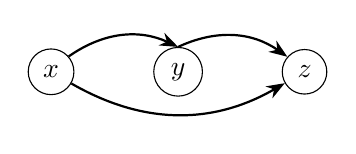
\begin{tikzpicture}[every node/.style = {draw, circle, minimum size = 10pt},
  relation/.style = {>=Stealth, ->, thick}]
  \node (x) [] {$x$};
  \node (y) [right = 1.0cm of x] {$y$};
  \node (z) [right = 1.0cm of y] {$z$};

  \draw [relation, bend left] (x) to (y.north);
  \draw [relation, bend left] (y.north) to (z);
  \draw [relation, bend right] (x) to (z);
\end{tikzpicture}
\end{document}

